%%% template.tex
%%%
%%% This LaTeX source document can be used as the basis for your technical
%%% paper or abstract. Intentionally stripped of annotation, the parameters
%%% and commands should be adjusted for your particular paper - title, 
%%% author, article DOI, etc.
%%% The accompanying ``template.annotated.tex'' provides copious annotation
%%% for the commands and parameters found in the source document. (The code
%%% is identical in ``template.tex'' and ``template.annotated.tex.'')

\documentclass[conference]{acmsiggraph}

\TOGonlineid{45678}
\TOGvolume{0}
\TOGnumber{0}
\TOGarticleDOI{1111111.2222222}
\TOGprojectURL{}
\TOGvideoURL{}
\TOGdataURL{}
\TOGcodeURL{}

\title{Adaptive Numerical CDF for Importance Sampling in BRDF}

\author{Diana Naranjo Pomalaya\thanks{e-mail:dnaranjo@ime.usp.br}\\IME - USP}
\pdfauthor{Diana Naranjo Pomalaya}

\keywords{global illumination, brdf, importance sampling, adaptive numerical cdf}

\begin{document}

%% \teaser{
%%   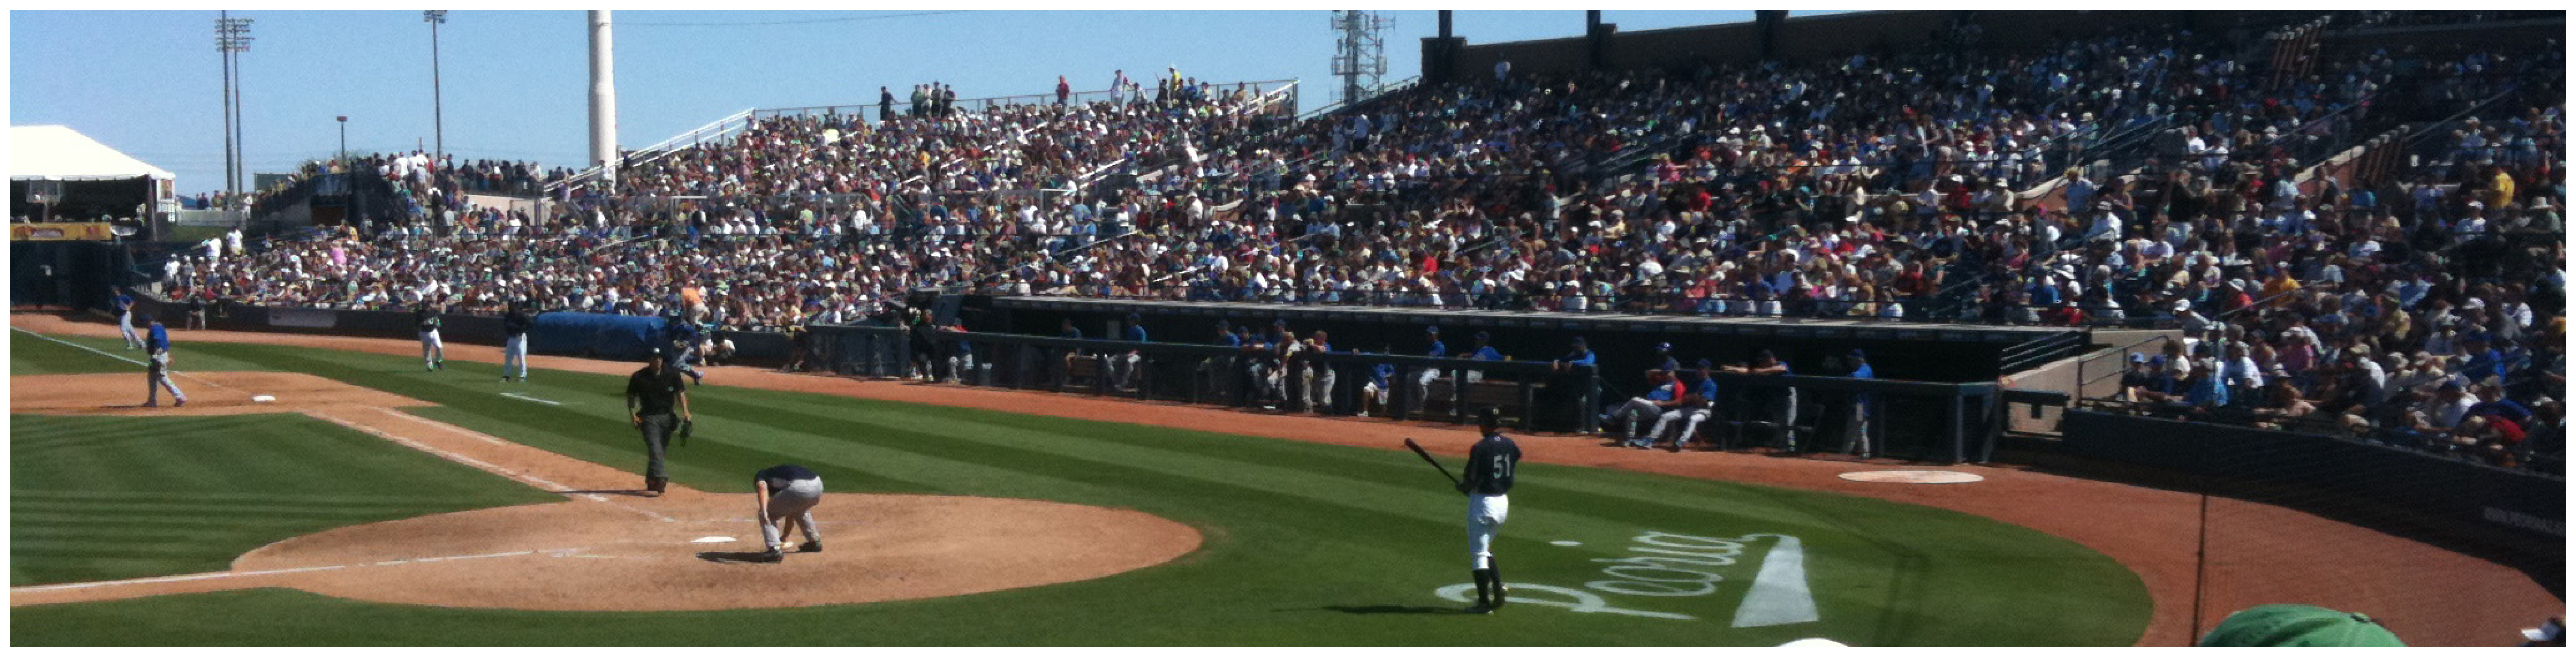
\includegraphics[height=1.5in]{images/sampleteaser}
%%   \caption{Spring Training 2009, Peoria, AZ.}
%% }

\maketitle

\begin{abstract}
Pbrt is a physically based ray tracing system that implements algorithms that enable photorealistic rendering, its goal is to render images indistinguishable from those taken from a camera. In the present implementation, the material class "MeasuredMaterial" is able to use measured data to compute the value of the Bidirection Reflectance Distribution Function (brdf) for any pair of incoming/outgoing directions. The use of real measured data leads to rendering realistic materials for the objects in scene. Currently, the method employed for sampling the incoming direction for a given outgoing one is: "Cosine-Weighted Hemisphere Sampling", which uniformly chooses an incoming direction based on the cosine term of the outgoing direction.~\cite{Pharr:2010:PBR} The main drawback of this approach is the lack of use of the information provided to the class about the distribution function. On the other hand, the amount of space needed to develop a CDF that would allow brdf sampling is as demanding as the amount to store the brdf itself or more. In the present project, a material and brdf class were developed. They employ the measured brdf data to create a CDF useful for brdf sampling. To avoid the space limitation constraint while maintaining the quality of the image rendered, a curve approximation algorithm was employed to create an adaptive CDF~\cite{Lawrence:2005:ANC}.
\end{abstract}

\copyrightspace

\section{Introduction}
Monte Carlo method, employed to compute the rendering equation, needs to draw random samples for the incident directions. To improve the result of the estimator, importance sampling has shown reduction in the variance. In the scattering equation the BRDF is weighted by a cosine term, this is why the "Cosine-Weighted Hemisphere Sampling" is a reasonable approach. The resulting sampling will most commonly generate directions nearer the top of the hemisphere, where the cosine term has a large value; rather than the bottom, where it becomes small~\cite{Pharr:2010:PBR}. However, the resulting distribution is still completely estranged from the material's reflectance function.

To generate a the CDF of the measured data we first realize that this function is represented by a piecewise-constant 2D function. The problem is we wish to sample an incident direction from an outgoing one and we have a function based on half-angle and difference vectors which depend on both incident and outgoing directions. The first needed to do is remap the values of the brdf to depend on the outgoing direction and another vector dependent on the incident direction, which is what we wish to sample. The simple answer would be to perform a re-parametrization to outgoing and incident vector. However, this representation requires a large amount of storage space~\cite{Lawrence:2004:EBI}. A different approach is the employment of the half-angle once again, since the BRDF presents a coherence for different outgoing directions and we wish to maximize the redundancy among slices of the function. The redundancy will lead to a greater compression later on.  

The goal of this project is to compress the amount of space required to represent a CDF that will enable a inversion sampling method for the reflectance function. This is accomplished by the means of a curve approximation algorithm performed over the CDF derived from the re-parameterized brdf dataset provided to the class.  The basic idea is that from a uniformly sampled CDF we generate an adaptive one which lifts the uniform restriction. The method used is the Douglas-Peucker greedy algorithm originaly employed for polygonal approximation of 2D curves~\cite{Douglas-Peucker:1973:AFT}.  This explanation takes place in a 1D CDF but it can be further generalized to multidimensional CDF which is the case of the brdf function. In the multidimensional case, a marginal 1D CDF is computed, then other conditional 1D CDF are computed by assuming one value of the previously sampled dimension and summing the rest. This approach is named “cascading CDF” by Lawrence~\cite{Lawrence:2005:ANC}.  

To demonstrate the benefits of the method employed we performed tests using different sets of BRDF data from the MERL database and measured the variations in Monte Carlo efficiency (variance divided by computation time) for different data sets and the amount of space saved by performing the compression.

\section{Background}
Monte Carlo is a numerical method that provides a solution that is statistically very likely to be close to the right answer. This is the method employed to compute the results to the integral equations that describe light scattering used in rendering. 
\begin{eqnarray}
L_{o}(p, \omega_{o}) = \int_{S^{2}}f(p, \omega_{o}, \omega_{i})L_{i}(p, \omega_{i})|cos \theta_{i}|d\omega_{i}
\end{eqnarray}
The expected value of the Monte Carlo estimator:
\begin{eqnarray}
\frac{(x_{1} - x_{0})(y_{1} - y_{0})(z_{1} - z_{0})}{N}\sum_{i}f(X_{i})
\end{eqnarray}
converges to the integral:
\begin{equation}
\int_{x_{0}}^{x_{1}}\int_{y_{0}}^{y_{1}}\int_{z_{0}}^{z_{1}}f(x, y, z)dxdydz
\end{equation}
and it's error decreases at a rate of $O(sqrt(N))$ in the number of samples taken. To be able to use the Monte Carlo estimator, it is necessary to be able to draw random samples from the chosen probability distribution of each of the random variables that compose the objective function. To do this one may use the inversion method, which maps uniform random variables to random variables from the desired distribution. To do this we need to have the Cumulative Distribution function of the random variable we wish to sample. Then invert the CDF and evaluate the inverse at a uniform random number $\varepsilon$.
In order to improve the result of the estimator one of the most effective method is to use importance sampling. It has been proven that to select a distribution that is similar to that of the integrand being estimated reduces the variance of the estimator which in turn improves the efficiency of estimator being used. It is called important sampling because samples are taken from the “important” part of the functions domain, i.e. where the function's value is relatively large~\cite{Pharr:2010:PBR}. 

The measured data of the reflectance function is 4-dimensional , 3-dimensional if the material is isotropic, that is presented in a tabular form. The MERL database, acquired by Matusik et al~\cite{Matusik:2003:ADR}, presents a list of brdf values based on the half-angle vector: $\omega_{h} = \widehat{\omega_{i} + \omega_{o}}$, where $\omega_{i}$ is the incident vector and $\omega_{o}$ is the outgoing vector; and the difference vector, which is computed by finding the rotation that aligns the half-angle vector with the (0,0,1) vector and then applying such rotation to the incident vector $\omega_{i}$. The data is indexed by $(\sqrt{\theta_{h}}, \theta_{d}, \phi_{d})$ where the number in each direction is 90, 90 and 180. The value of difference phi is dropped due to the isotropic behavior of the materials. The square root is taken in order to increase the the sampling rate for theta half close  to zero, where the cosine term preciously mentioned is higher~\cite{Pharr:2010:PBR}. As stated before we need to re-parameterize this function to outgoing and half-angle directions to generate an inversion sampling useful CDF.  This remapping consists in a list of values in a tabular form indexed by a number of outgoing theta and phi values (each number independent) and a number of half-angle theta and phi values (also independent). The sampling can then be performed by sampling a 2D distribution (half-angle) based on the outgoing direction given as an input.

\begin{equation}
(\sqrt{\theta_{h}}, \theta_{d}, \phi_{d}) \rightarrow (\theta_{o}, \phi_{o}, \theta_{h}, \phi_{h})
\end{equation}

We are thus interested in the case of piecewise-constant 2D distributions which is implemented in pbrt's current version. To explain how this works we first explain how does the piecewise-constant 1D distribution inversion method sampling works. We assume that we have a 1D function split into N equal-sized pieces (size = 1/N) as shown in Figure 1 (a). The function's value in each of the regions is a constant. 

\begin{figure}[ht]
  \centering
  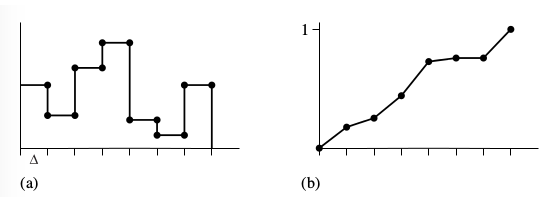
\includegraphics[width=3.5in]{images/piecewise}
  \caption{(a) Piecewise-constant function. (b)Piecewise-linear cdf.}
\end{figure}

The integral of this function is the sum of all the constants weighted by the size of the region. Since this size is 1/N for all the regions then the integral becomes the sum of all the values of the function divided by the number of regions. The PDF of the function then should be $f(x)/funcInt$, where funcInt is the function's integral. The CDF can be then computed as a list of values (N + 1), as shown in Figure 1 (b) and given an $\varepsilon$ random number we can perform a binary search that tracks the region where this value is $P(x_{i}) \leq \varepsilon$ and $\varepsilon \leq P(x_{i+1})$~\cite{Pharr:2010:PBR}.

The 2D case is a bit more complex, we assume we have a function $f(u, v)$ defined by a list of nu x nv values. The integral of f is the sum of all $f(u_{i}, v_{j})$ values divided by $n_{u}$ x $n_{v}$, i.e. number of regions. We then define the PDF of f a the value of the function $f(u, v)/funcInt$, where funcInt is once again the function's integral. To translate this problem to the previously solved 1D situation we generate the marginal density $p(v)$, which can be obtained by:

\begin{equation}
p(v) = \int p(u,v)du = \frac{(1/n_{u})\sum_{i}f[u_{i},\tilde{v}]}{funcInt}
\end{equation}

where $\tilde{v}$ represents the region to which v belongs. We can now solve this problem using the 1D method explained before since it is a piecewise-constant 1D function. We can now explain the second step which is the conditional density $p(u|v)$:

\begin{equation}
p(u|v) = \frac{p(u,v)}{p(v)} = \frac{f[\tilde{u}, \tilde{v}]/funcInt}{p[\tilde{v}]}
\end{equation}

where $\tilde{u}$ and $\tilde{v}$ represent the regions to which $u$ and $v$ belong. This is also a piecewise-constant 1D function and can also be solved in a similar way as the marginal distribution. To solve the 2D case we will then have one 1D marginal distribution and $n_{v}$ 1D conditional distributions~\cite{Pharr:2010:PBR}. 

One final consideration is the transformation performed from incident direction to the half-angle one. We have a CDF of the half-angle vector based on the outgoing vector, but we wish to sample an incident direction. This is the same as to having a random variables $x_{i}$ drawn from some PDF $p(x)$ and wish to find the distribution of a new random variable $Y_{i}$, where $Y_{i} = f(x_{i})$. To change the density in term of the half-angle vector to one in terms of incident vector we must apply the adjustment for a change of variables. By the spherical coordinate system oriented about the outgoing vector we obtain:

\begin{equation}
\frac{d\omega_{h}}{d\omega_{i}} = \frac{sin\theta_{h}d\theta_{h}d\phi_{h}}{sin\theta_{i}d\theta_{i}d\phi_{i}}
\end{equation}

because $w_{i}$ is computed by reflecting $w_{o}$ about $w_{h} = \theta_{i} = 2\theta_{h}$. Plus, since $\phi_{i} = \phi_{h}$ we find that:

\begin{equation}
\frac{d\omega_{h}}{d\omega_{i}} = \frac{1}{4(\omega_{o}\cdot \omega_{h})}
\end{equation}

And thus the PDF after transformation is:
\begin{equation}
p(\theta, \phi) = \frac{p_{h}(\theta, \phi)}{4(\omega_{o}\cdot \omega_{h})}
\end{equation}

\section{Multidimensional Numerical CDF Compression}
Once we have the 1D uniformly spaced CDFs we can initiate the step of compression. In order to obtain an adaptive CDF we use a polygonal curve approximation algorithm. This algorithms take as input a curve represented by N points and returns M, where those M are selected so as to minimize the error between the two curves and using as few as possible points. The algorithm employed in this case does not return the optimal solution but returns an answer approximately correct (80\% accuracy). This is the Douglas-Peucker greedy algorithm, which was selected due to its speed and simplicity~\cite{Douglas-Peucker:1973:AFT}. 

The basic idea of the algorithm is the following: we initiate our representation of reduced curve by adding the first and last point of the original curve, then we enter a loop where we pick the furthest point from the curve we already have (at the beginning the line from init point to last point). The loop terminates when a limit to the number of points that represent the reduced curve is achieved or when the distance of the furthest point to the reduced curve is less that some $\varepsilon$. The number of maximum point that represent the reduced curve and the value of $\varepsilon$ are parameters that represent this algorithm~\cite{Lawrence:2005:ANC}.  The illlustation of how does the Douglas-Peucker algorithm work is shown in Figure 2.

\begin{figure}[ht]
  \centering
  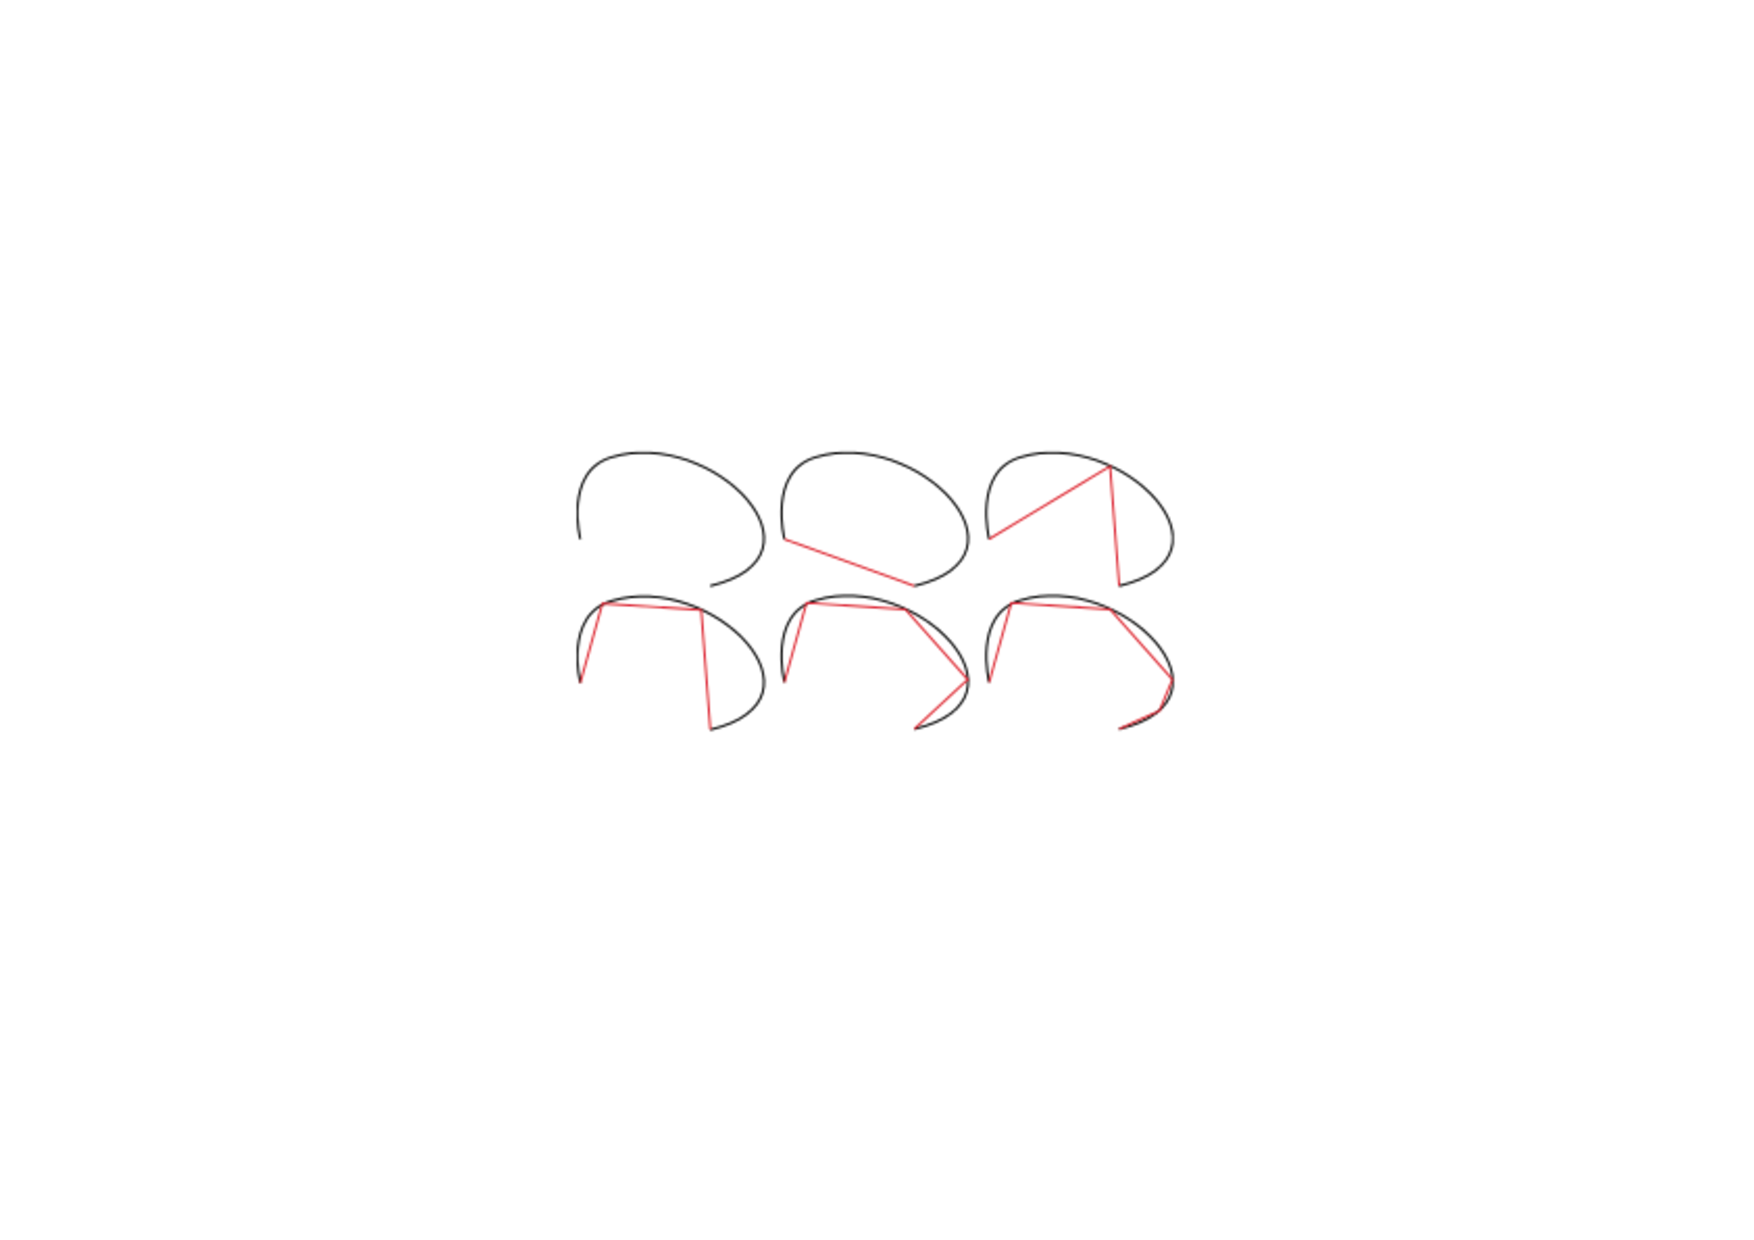
\includegraphics[width=3.5in]{images/curveApproximation}
  \caption{Douglas-Peucker algorithm.}
\end{figure}

The application of this algorithm to the 1D CDFs is direct. Once the algorithm is applied to the uniform 1D CDF we directly obtain the adaptive CDF and can therefore use it to perform the inversion method to perform the sampling. This sounds simple enough, but it deceptively hides some necessary intermediate steps. To compute the 1D uniform marginal distribution we must first compute the conditional distributions and thus we find that the first step is to generate the complete 2D structure as an intermediate step. However, this required space will only be needed for the initial part (before the renderization step initiates) and thus will not present a problem later on. Once we have the required uniform marginal distribution we can apply the compression algorithm thus obtaining an adaptive marginal distribution. The next step is to compute the conditional distributions for the newly generated un-uniformly spaced regions. The conditional CDF will then be the average across its associated range~\cite{Lawrence:2005:ANC}:

\begin{equation}
 p(u|v_{i}) = \frac{1}{|v_{i}|} = \int_{v_{i-1}}^{v_{i}}\frac{p(u, v')}{p(v')}
 \end{equation}

With this newly computed distribution functions we generate new 1D uniform conditional distributions. Then we apply the compression algorithm for each one of the regions generated by the adaptive marginal. 

In pbrt it is important to implement not only the sampling function method “Sample\_f” for new brdf classes but also the “Pdf” function, which returns the value of the PDF for an arbitrary given direction. This method is useful for multiple importance sampling, and thus it is important that “Sample\_f” and “Pdf” return consistent results. One important difference with the uniformly spaced CDF is the cost of evaluating this probability. The cost in the uniform situation is $O(1)$ thanks to its uniformity, whereas the adaptively spaced CDF requires $O(log N)$, where N refers to the number of non-uuniform samples that represent the CDF. This increment in the cost is due to the need to perform a binary search over the values of the function to find the region that represents it. Since the whole idea of compression is to obtain a really small N then this newly acquired cost turns insignificant.  The cost for generating a sample remains the same as in the uniform case, which is $O(log N)$, but it must be remembered that N in the adaptive case is much smaller than N in the uniform one. 

\section{Results}
We now present the results of the sampling from the compressed adaptive CDF compared to sampling from the uniformly spaced CDF. In order to do this we performed tests using the following sets of BRDF data from the MERL database: Nickel, Plastic and Metallic-Blue. We focus on glossy materials instead of diffuse ones because the first benefit more from sampling according to the distribution of energy in the BRDF. We then perform a comparison in the Monte Carlo efficiency, variance divided by computation time, for the different data sets. We also measure the amount of space saved by performing the compression. The uniformly-sampled CDF has a resolution of 32 x 16 x 256 x 32 $(\theta_{o}, \phi_{o}, \theta_{h}, \phi_{h})$ which lead to near 4 million samples of the distribution function. The corresponding adaptive numerical CDFs have an average resolution of 32 x 16 x 30 x 26 taking this value down to 400 thousands. The compression thus presents a rate of 10:1. 

Table 1 presents the results of the experiments, the original resolution of the CDF, the average resolution of the adaptive CDF, compression ratio and the Monte Carlo efficiency measures of both the original and adaptive CDF samplings. We can observe that the efficiency measures are very similar between the uniform resolution and the adaptive one. Thus, we can conclude that the quality of the image remains the same while saving 10 times storage cost.

\begin{table}[ht]
  \centering
  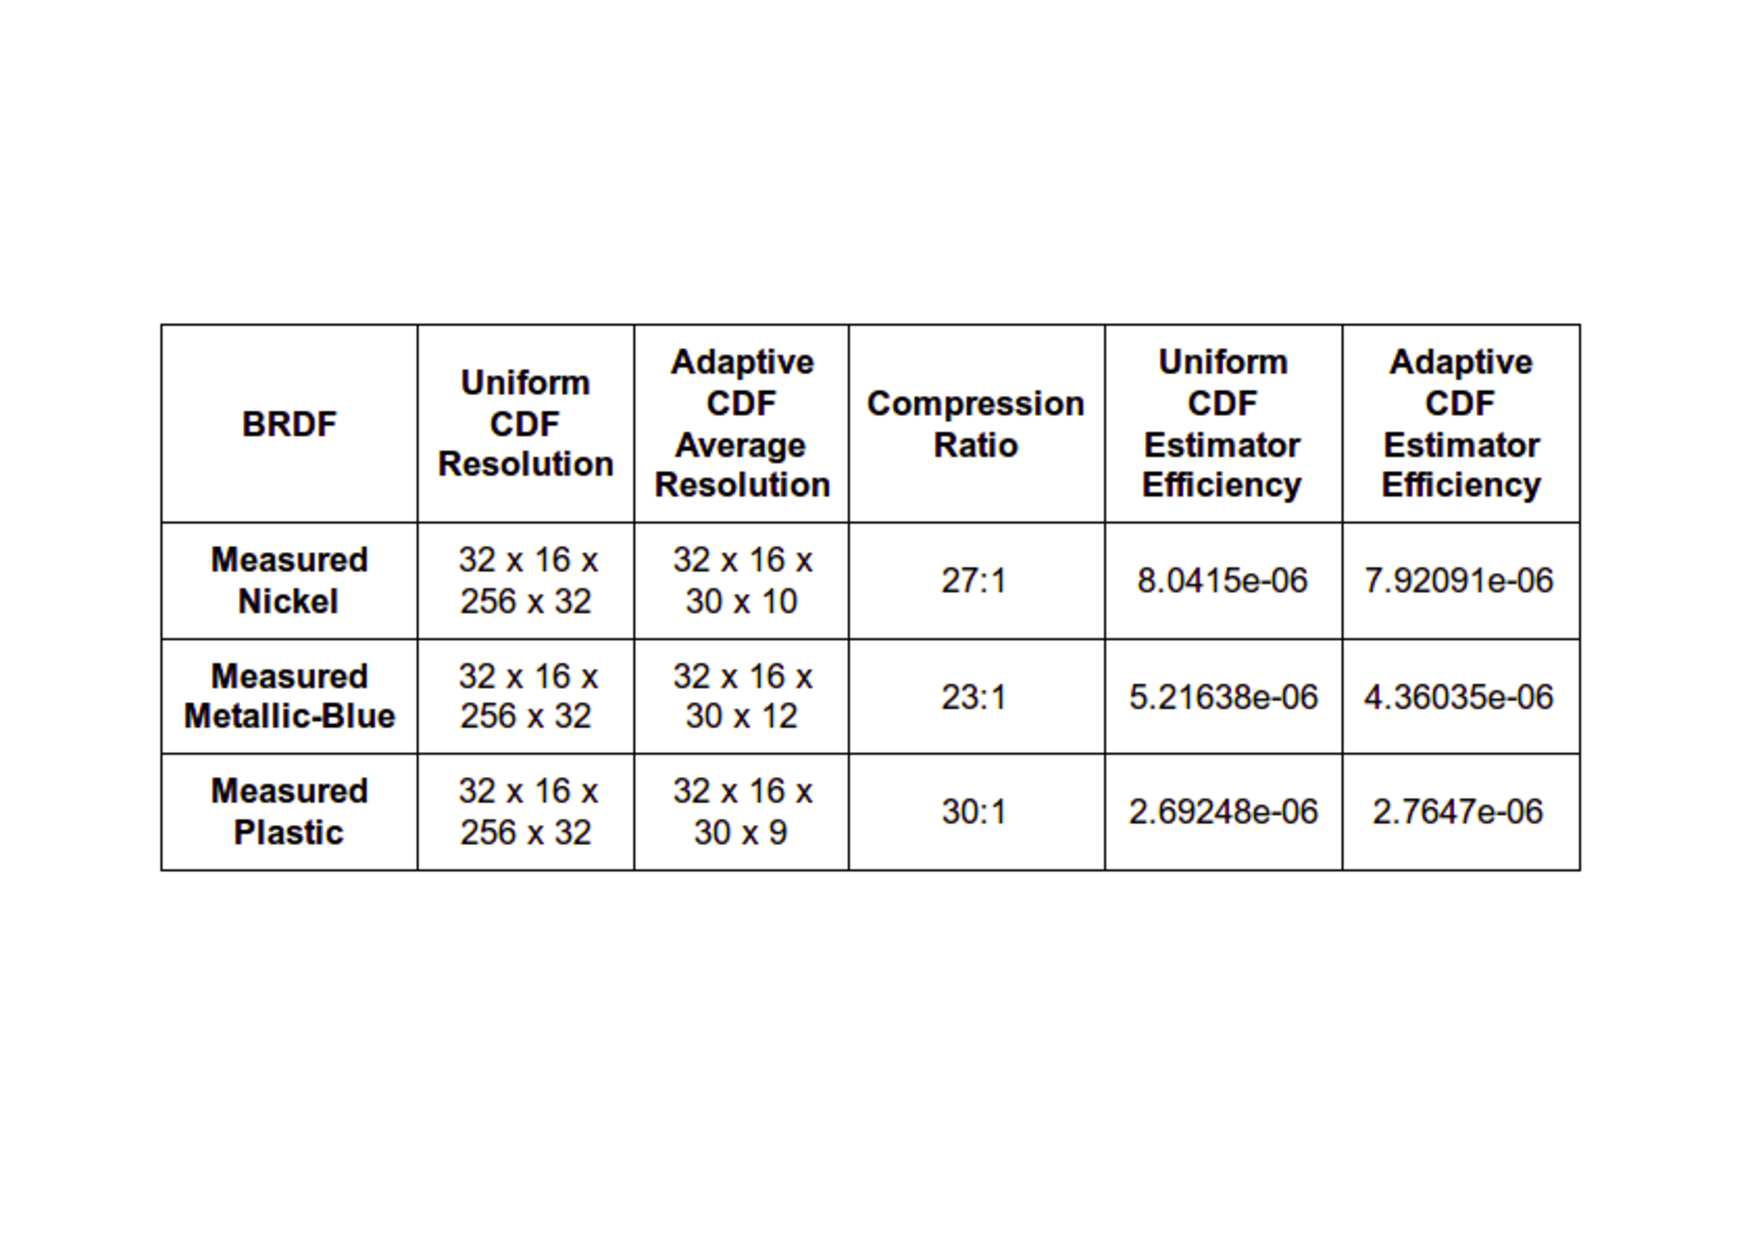
\includegraphics[width=3.5in]{images/results}
  \caption{Experiment Results}
\end{table}

Table 2 presents the rendered images obtained by performing reflectance sampling employing the uniformly spaced cdf and the adaptive cdf on the measured nickel, metallic-blue and plastic brdfs. The third colum shows the difference between them. The areas with red shadings are the pixels that present a greater difference between the two rendered images. Meanwhile, the white areas represent the pixels that present no change between them. As it can be observed, the areas where the difference is greater are those around the highlights  

\begin{table}[ht]
  \centering
  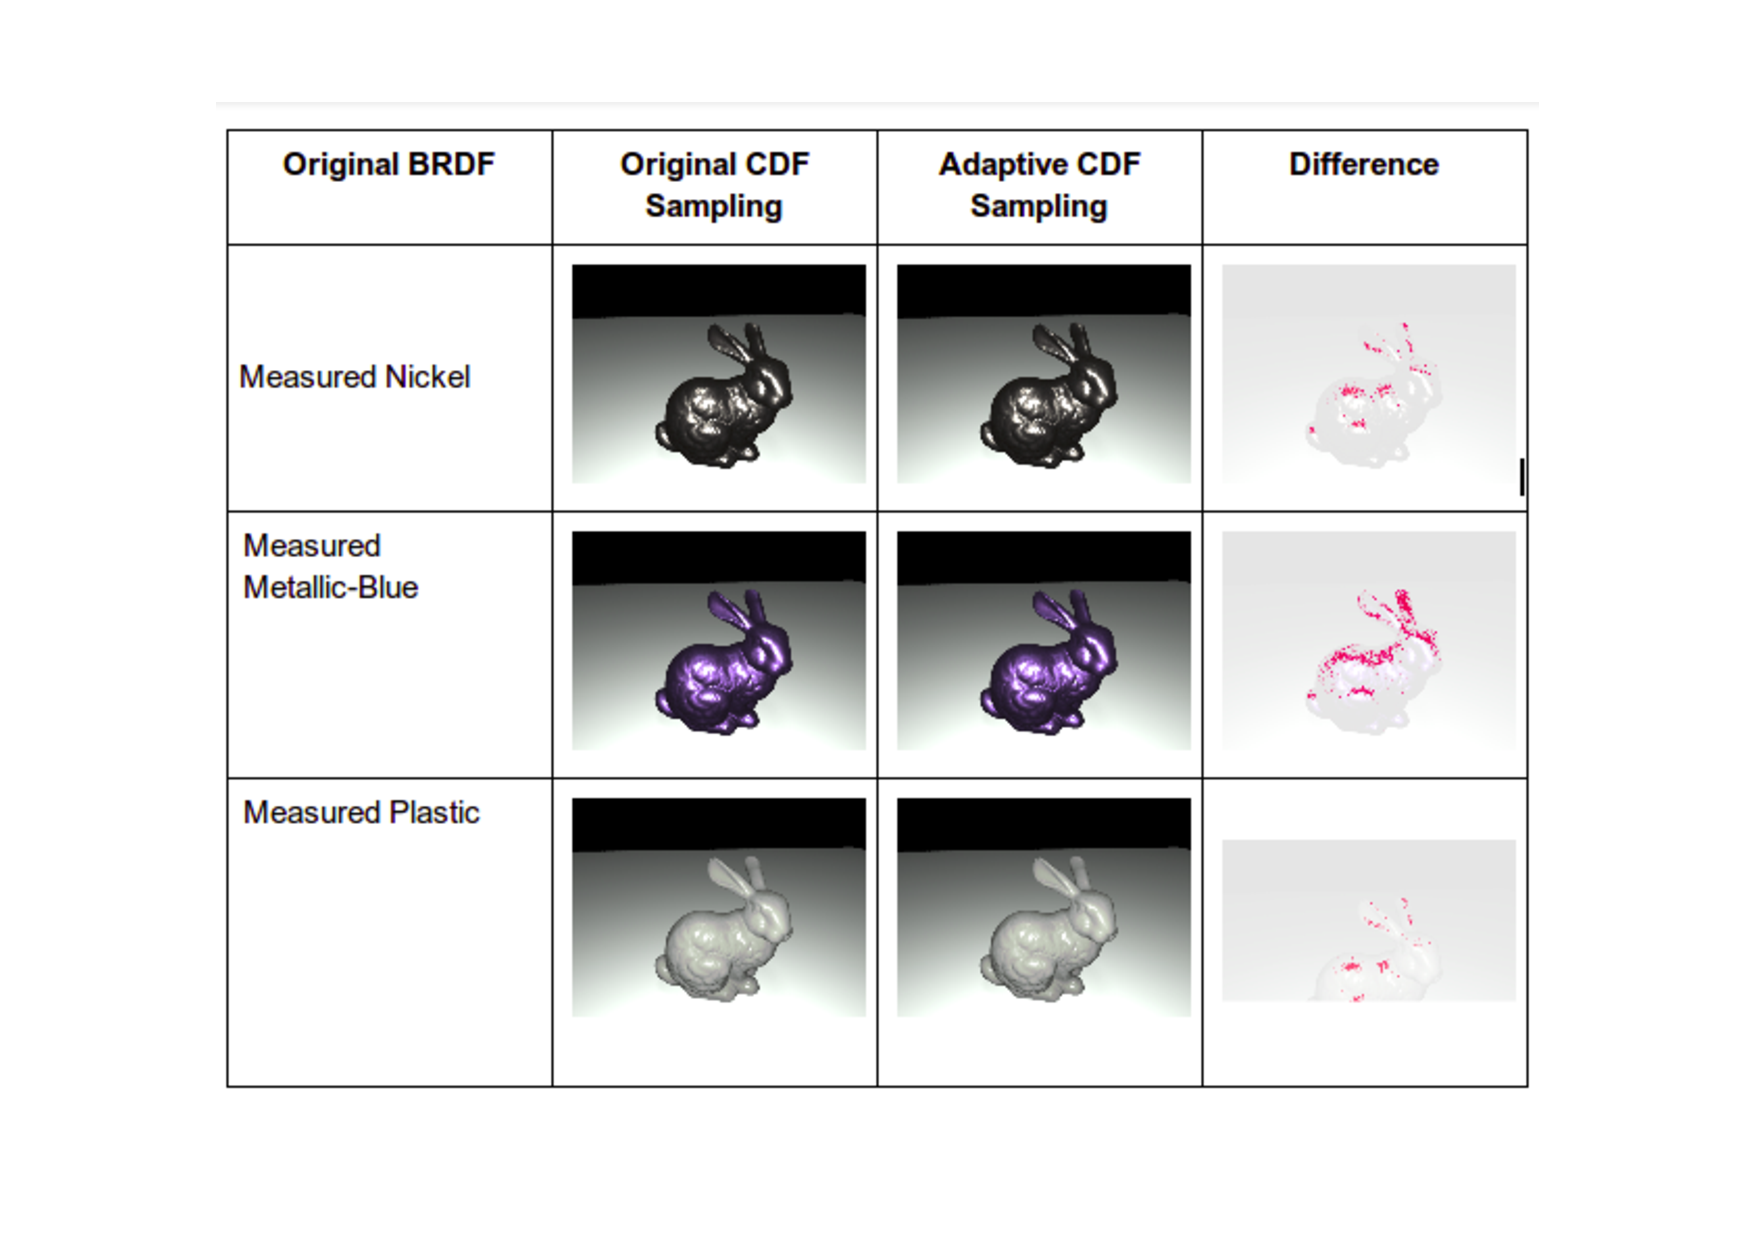
\includegraphics[width=3.5in]{images/resultsImages}
  \caption{Rendered Images and Difference between uniform and adaptive CDFs}
\end{table}

\section{Conclusions and Future Work}
This project is related to the problem of efficient importance sampling based on the measured BRDF. We have applied a known curve approximation algorithm to compress the size of the CDF for importance sampling. By the results obtained in the experiments we can conclude that the employment of such an algorithms results in a significant reduction of storage cost while maintaining the quality of the original CDF. However, more compression might be accomplished if a higher dimensionality is employed and the outgoing angles are also spaced in an adaptive form instead of uniform as is the case in the present project.

As stated in the paper that inspired the present project~\cite{Lawrence:2005:ANC} this algorithm can be employed in local environment map sampling, which is a form of representing the illumination. Currently, some light classes employ environment maps and uniformly spaced distributions to represent them. However, if this distributions were exchanged for those of the adaptive form we might be able to obtain the same results while saving some storage cost and thus have the possibility of developing more complex scenes.

\section*{Acknowledgements}

This work was achieved thanks to the available MERL database, documentation of the pbrt system and the support of Jose Miguel Noblecilla.  

\bibliographystyle{acmsiggraph}
\bibliography{document}
\end{document}
